% [R40] Subsection-by-subsection terminology and handbook alignment; see revisions/REVISION_R40.md.
\section{Corpus and Annotation}
\label{sec:framework}

\subsection{Task Definition and Label Schema}

Given a Chinese job-advertisement sentence $x$, the task is to predict non-overlapping spans $(s,e,t)$, where $t\in\{L,K,S,T\}$. Offsets are measured in Unicode code points: $s$ denotes the zero-based start position, and $e$ denotes the exclusive end position. Each annotated mention must match the contiguous substring $x[s:e]$ exactly, including its spelling and internal spaces. The annotations describe requirements stated in the advertisement, not an applicant's actual abilities.

\begin{figure}[!htbp]
  \centering
  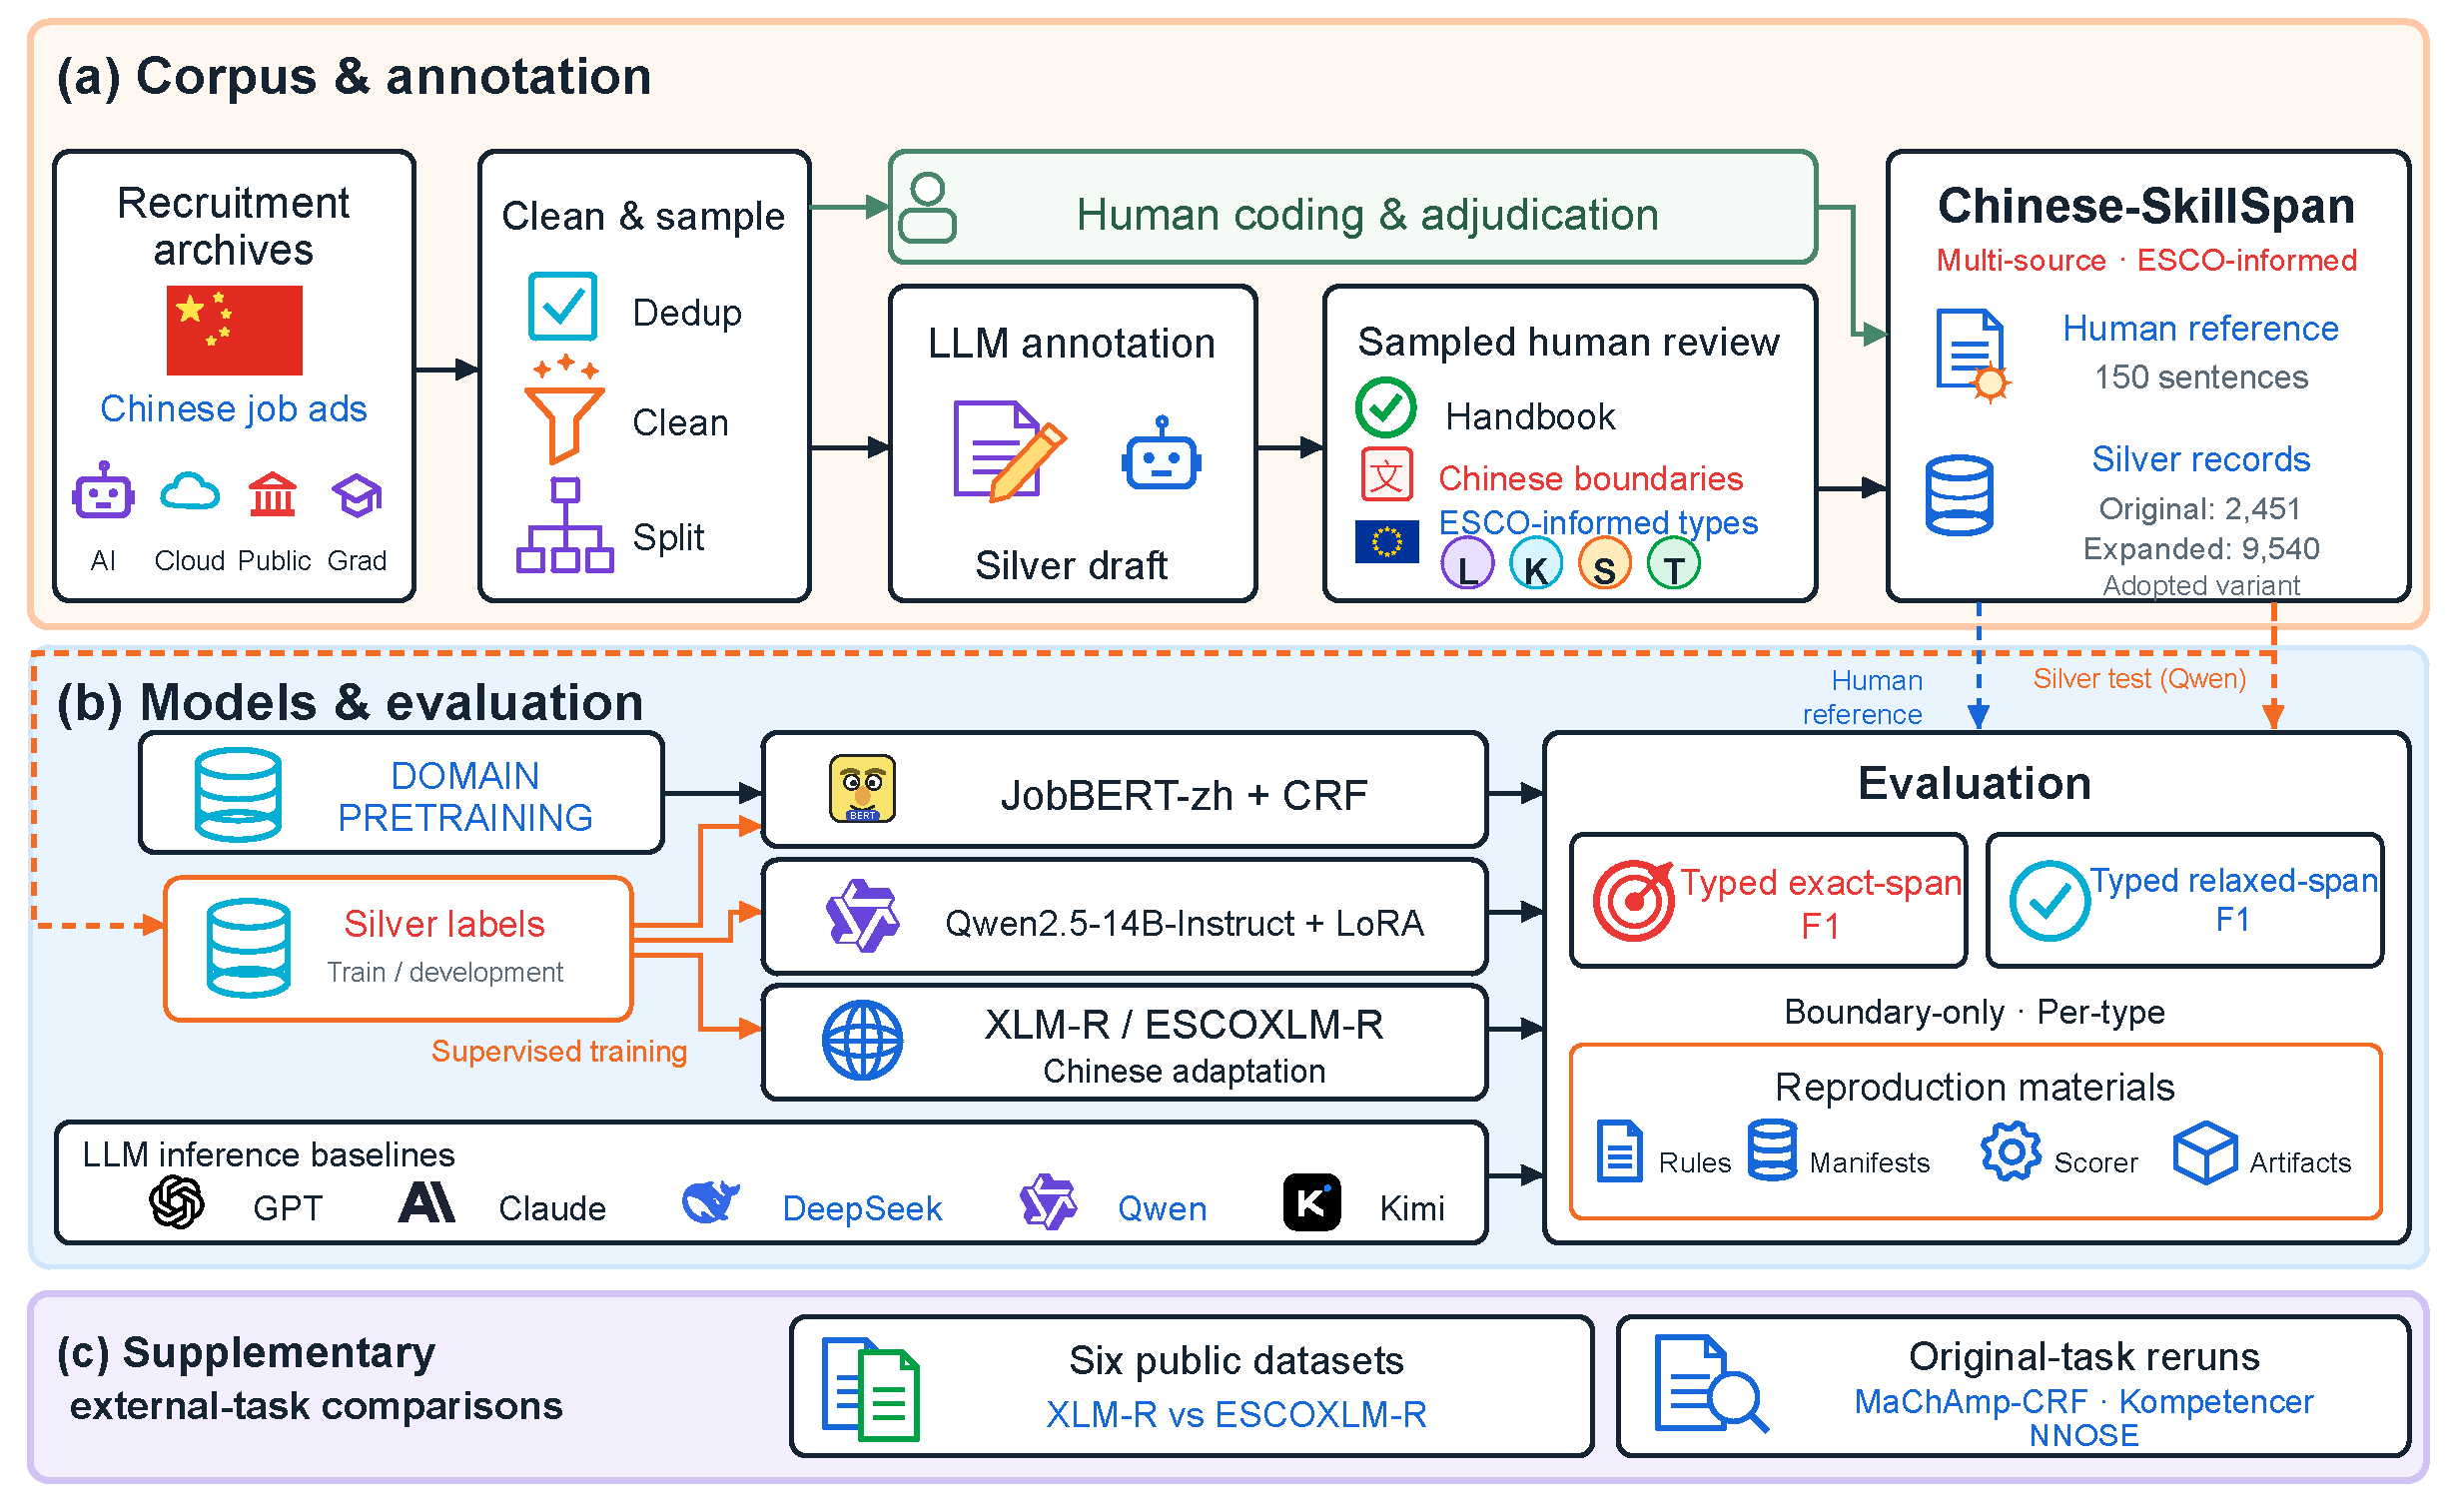
\includegraphics[width=\textwidth]{figures/Figure1_drawio_restored_20261004.pdf}
\caption{Overview of Chinese-SkillSpan: (a) corpus preparation and annotation; (b) model training and evaluation; and (c) supplementary external-task comparisons. Initial layout assisted by OpenAI image generation; final vector drawing prepared with Codex-assisted code (\hyperref[app:d]{Appendix~D}).}
  \label{fig:macro-micro}
\end{figure}

Figure~\ref{fig:macro-micro} summarizes corpus preparation, annotation, and model evaluation. The four categories in Table~\ref{tab:guide-types} draw on ESCO and the knowledge--skill distinction in the European Qualifications Framework~\citep{ESCOv1_2_2024,council2017eqf}.

The definitions and rule examples below illustrate the current handbook, v4.2.14, also used in the blinded agreement study. The human reference retains v4.2.10 labels, whereas the original bulk-generation prompt follows v4.2.12. Current examples do not revise historical annotations; \hyperref[sec:guide-version-history]{Appendix A.4} documents the version boundaries.

\begin{table}[!htbp]
\caption{Operational L/K/S/T definitions and illustrative Chinese spans under handbook v4.2.14.}
\label{tab:guide-types}
\centering\small
\setlength{\tabcolsep}{4pt}
\renewcommand{\arraystretch}{1.12}
\begin{tabularx}{\linewidth}{@{}P{0.19\linewidth}P{0.47\linewidth}L@{}}
\toprule
Label & Operational definition & Chinese examples and English glosses \\
\midrule
L: Language & Natural-language names, proficiency levels, examinations, and certificates. & \zh{英语六级}\par\emph{College English Test Band 6}\par\smallskip\zh{日语N2}\par\emph{Japanese proficiency at N2 level} \\[3pt]
K: Knowledge-related requirements & Facts, principles, theories, and fields of study; educational and non-language qualifications; and explicit industry-background requirements. & \zh{SQL原理}\par\emph{Principles of SQL}\par\smallskip\zh{本科及以上学历}\par\emph{Bachelor's degree or higher} \\[3pt]
S: Occupational skill & Occupational activities and the application of tools or methods. & \zh{使用}[\zh{SQL}]\par\emph{Use [SQL]}\par\smallskip\zh{数据分析}\par\emph{Data analysis} \\[3pt]
T: Transversal competency & General communication, cooperation, cognition, self-management, and dispositions. & \zh{客户汇报}\par\emph{Reporting to clients}\par\smallskip\zh{责任心}\par\emph{Sense of responsibility} \\
\bottomrule
\end{tabularx}
\end{table}


K combines substantive knowledge with recruitment proxies by project convention; qualifications and industry background are not treated as measures of knowledge under ESCO or the EQF. Its scores therefore describe this combined category. The frozen labels do not distinguish these subtypes, so a knowledge-only evaluation would require additional human review.

\begin{figure}[htbp]
\centering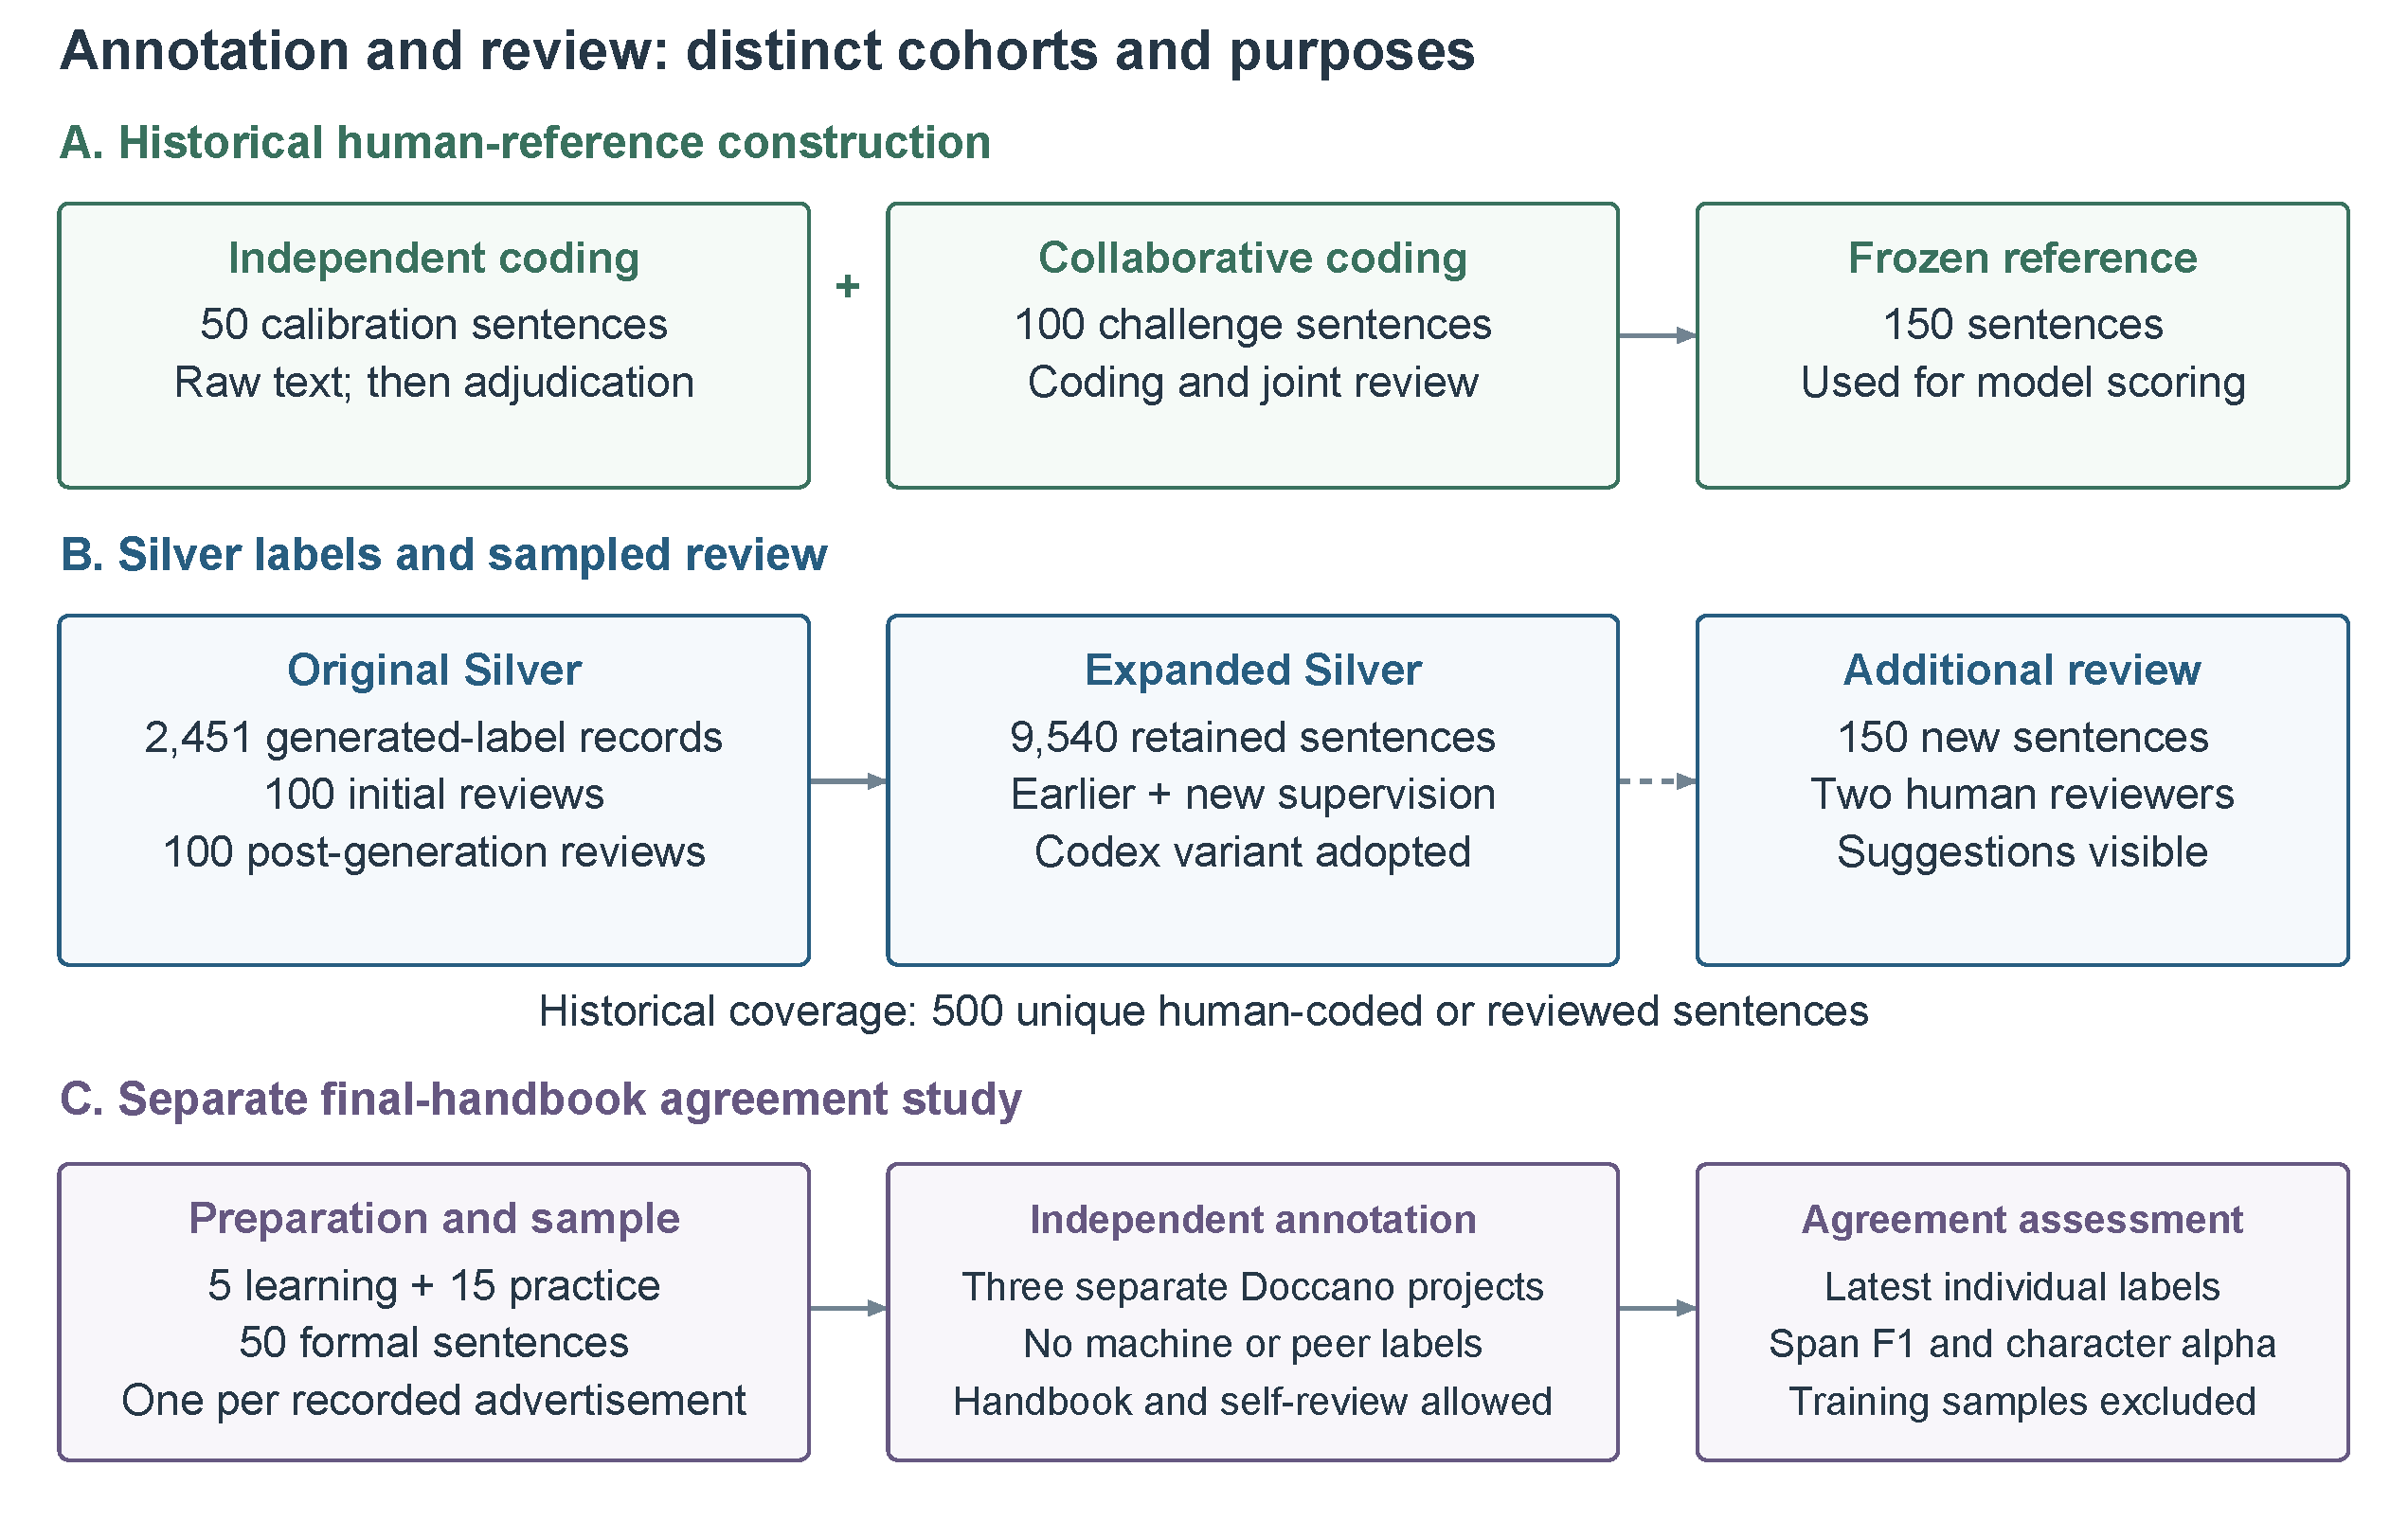
\includegraphics[width=\linewidth]{figures/annotation_paths_major_revision_20261004.pdf}
\caption{Annotation cohorts and their roles. Historical coding and review cover 500 unique sentences. The separate agreement study uses the latest individual annotations after self-review; its five learning and 15 practice sentences are excluded from agreement.}
\label{fig:coding-detail}
\end{figure}


\subsection{Data Sources and Annotation Layers}
\label{sec:challenge-audit}

The source corpus contains 22,840 sentences from four collection batches: AI, Cloud, public-sector, and graduate recruitment. Texts came from commercial collections purchased from MacroData~\citep{macrodataPlatform}, public-institution announcements collected by the research team, and the Recruitment Dataset on Alibaba Cloud Tianchi~\citep{tianchiRecruitment163746}. For the public-institution subset, the team selected government, university, hospital, and public recruitment websites across China, then screened and cleaned the collected texts. The batches can overlap in occupational coverage.

Table~\ref{tab:annotation-lineage} summarizes the principal annotation layers and their uses, following guidance on dataset documentation~\citep{bender2018datastatements,gebru2021datasheets}. The human reference provides evaluation labels, while records selected from the original silver pool provide training and development labels. The adopted expanded silver pool combines earlier supervision with additional cloud, public-sector, and listed-company recruitment texts selected using requirement-related keywords. The model-specific training and development splits are described in \nameref{sec:experiments}.

\begin{table}[!htbp]
\caption{Source corpus and principal annotation layers in Chinese-SkillSpan.}
\label{tab:annotation-lineage}
\centering\small
\setlength{\tabcolsep}{4pt}
\begin{tabularx}{\linewidth}{@{}P{0.20\linewidth}P{0.18\linewidth}P{0.31\linewidth}L@{}}
\toprule
Subset & Size & Annotation content & Role \\
\midrule
Source corpus & 22,840 sentences & Recruitment text from four collection batches & Source material for annotation \\
Human reference & 150 sentences & 663 spans; 8 sentences with no spans (5.3\%) & Model evaluation \\
Original silver pool & 2,451 records & Model-generated annotations with sampled human review & Candidate supervision \\
Adopted expanded silver & 9,540 records & 21,101 spans; 2,492 records with no spans (26.1\%) & Expanded supervision and evaluation against silver targets \\
\bottomrule
\end{tabularx}
\par\smallskip
{\footnotesize\RaggedRight Pool sizes count annotation records, which may repeat a sentence. The layers overlap in source material and should not be summed.\par}
\end{table}

The human reference contains 663 spans: 448 S, 125 K, 88 T, and two L. The 150 sentences have distinct complete texts after Unicode Normalization Form C (NFC). This operation gives equivalent character sequences a consistent representation for comparison. An alternative expanded pool contains 9,646 records and supports a supplementary annotation-channel comparison. \hyperref[app:d]{Appendix D} details both expanded pools' source partitions, composition, and \mbox{selection criteria}.


\subsection{Annotation Guidelines and Adjudication}
\label{sec:annotation-guidelines-r36}

Scope is determined clause by clause. Benefits, application procedures, company promotion, and outcomes alone are excluded; recruitment activities may qualify when they are occupational duties. Thus, \zh{五险一金} (social insurance and housing fund benefits) receives an empty annotation, whereas \zh{能力提升} (capability improvement) without sufficient context remains unresolved. Confirmed absence of an in-scope mention is distinguished from missing context or uncertain interpretation, including in mixed clauses.

Boundary selection prioritizes semantic completeness. Following SkillSpan~\citep{zhang2022skillspan}, annotators retain the shortest complete source span, with no fixed length limit or added words. Generic proficiency triggers usually remain outside the span, but necessary heads and complements remain inside; \zh{会聊天} (can converse) retains its modal as a complete capability expression. Coordinated items are split only when each remains interpretable in context. For example, \zh{熟悉使用Word，Excel，PPT等办公软件} (familiar with office software such as Word, Excel, and PowerPoint) permits separate Word, Excel, and PPT spans. In contrast, \zh{优化曝光与转化率} (optimize exposure and conversion rate) remains one S span because the objects require the shared optimization action.

Experience wording is assessed by distinguishing occupational activities, generic tenure, and industry background. Generic duration alone is excluded; explicit industry-background requirements receive the project-specific K label. For a named activity, annotators remove the experience qualifier only if the remaining words still express the requirement in context. Thus, \zh{机器人竞赛经验} (robotics competition experience) retains its qualifier when the bare event name would change the requirement. Coordinated items must each pass the same test. \hyperref[app:a]{Appendix A} illustrates how internet-company operations receive S while an industry-background requirement receives K.

Type depends on the requirement in context: \zh{使用SQL} (use SQL) supports S for SQL, whereas \zh{了解SQL原理} (understand SQL principles) supports K for \zh{SQL原理} (SQL principles). A predicate can determine type while remaining outside the span; familiarity alone does not determine type. General communication and coordination receive T even in duty clauses, whereas technical operations receive S. Adjudication resolves scope, boundaries, and type separately, without a global label priority~\citep{artstein2008agreement}. Once scope and boundaries are resolved, type-only uncertainty may receive provisional S in the working record, with alternatives logged. All records with unresolved uncertainty are excluded in full from final training targets; provisional S is not an accepted default. Alternative annotations, nested candidates, and unresolved overlaps remain separate from the final flat layer. Figure~\ref{fig:illustrative-annotations} shows frozen human-reference examples; \hyperref[app:a]{Appendix A} retains the complete G1--G15 rules.

\begin{figure}[!htbp]
\centering
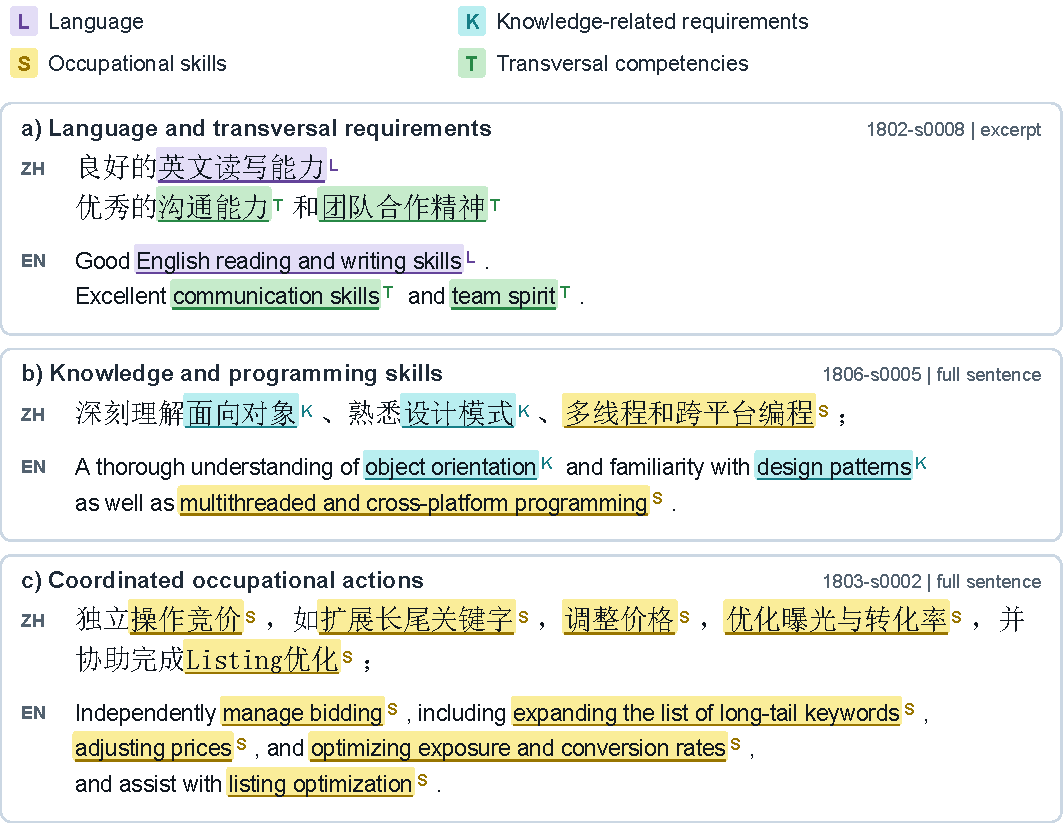
\includegraphics[width=\linewidth]{figures/annotation_examples_main_20261006.pdf}
\caption{Chinese human-reference spans with aligned English translations. Matching colors and labels indicate span correspondences; Chinese highlights reproduce the original reference labels (metadata: v4.2.10).}
\label{fig:illustrative-annotations}
\end{figure}


\subsection{Human Annotation and LLM-Assisted Labeling}
\label{sec:annotation-workflow-r36}

Human annotation, review, and adjudication established the human reference set and informed handbook development. The LLM-labeling route in Figure~\ref{fig:macro-micro} concerns Silver supervision. The adopted annotation route used the official OpenAI Codex interface. In this paper, Codex identifies the interface; Table~\ref{tab:model-identity} lists the recorded model names and their roles. An initial sample review preceded bulk annotation. Automated checks examined span text, offsets, labels, and record coverage, while sampled human review assessed the interpretation of requirements. Each annotation batch used the handbook version available at the time of generation, with later amendments documented separately.

In the adopted expanded-Silver variant, annotations for the designated replacement subset were generated through Codex. Earlier supervision components were retained in both pools, and the alternative variant is reported as a supplementary comparison. Appendices~A~and~D document the handbook versions, record-inclusion decisions, and exclusion of unresolved records.

\FloatBarrier

\subsection{Annotation Quality and Reference Freezing}
\label{sec:annotation-quality}

Agreement must be measured without shared suggestions if it is to assess how consistently annotators apply the handbook. We therefore report the independent blinded study in Table~\ref{tab:quality-main}. Historical coding and assisted-review studies used different samples and rules; their scores cannot be read as a longitudinal improvement in independent reliability (\hyperref[app:b]{Appendix B}).

\paragraph{Blinded coding protocol.}
Three annotators used handbook B.sop\_v4.2.14 after familiarization and training on sets of five and 15 sentences, following the training-and-feedback approach discussed by \citet{klie2024annotationquality}. They then independently coded the same random sample of 50 Silver teacher-pool sentences in separate Doccano projects, blinded to both machine suggestions and one another's labels. Training sentences are excluded from formal agreement. The sample contains one sentence from each of 50 recorded advertisement identifiers; it assesses annotation agreement and is not a new model test set. Source counts and sampling-record limits appear in \hyperref[app:b]{Appendix B}.

We computed agreement from the preserved pre-discussion exports, retaining all 50 sentences and all three coder pairs. Typed exact F1 measures agreement on complete spans without designating a coder as gold~\citep{hripcsak2005agreement}; boundary-only F1 ignores type. Nominal Krippendorff's $\alpha$ uses L/K/S/T/O assignments to all 2,111 source code points. Percentile 95\% intervals use 10,000 source-stratified sentence-bootstrap samples, retaining all three annotations together. These intervals condition on the observed source mixture and coders.

\begin{table}[htbp]
\caption{Independent blinded agreement among three annotators on 50 sentences. Character coefficients are Cohen's $\kappa$ unless marked $\alpha$. Brackets give 95\% bootstrap intervals for typed exact F1. ``Equal'' counts identical sentence-level span sets. Training samples are excluded.}
\label{tab:quality-main}
\centering\small
\begin{tabularx}{\linewidth}{@{}p{0.22\linewidth}rp{0.09\linewidth}p{0.21\linewidth}L@{}}
\toprule
Comparison & $n$ & Character & Typed F1 & Details \\
\midrule
\multicolumn{5}{@{}l}{\textit{Final-handbook independent blinded coding}} \\
A--B & 50 & 0.800 & \makecell[l]{0.657\\{}[0.528, 0.767]} & Boundary F1 0.762; equal 26/50 \\
A--C & 50 & 0.848 & \makecell[l]{0.739\\{}[0.612, 0.850]} & Boundary F1 0.788; equal 33/50 \\
B--C & 50 & 0.803 & \makecell[l]{0.594\\{}[0.459, 0.717]} & Boundary F1 0.721; equal 22/50 \\
Mean / three-rater & 50 & $\alpha$ 0.817 & \makecell[l]{0.663\\{}[0.562, 0.759]} & Mean boundary F1 0.757; all three equal 21/50 \\
\bottomrule
\end{tabularx}
\end{table}

Independent blinded coding leaves substantial span-level disagreement. Mean typed F1 is 0.663, below the planned 0.80 project target, which is not a universal reliability cutoff. Boundary F1 is higher at 0.757 (95\% CI [0.654, 0.846]), indicating additional type disagreement. Character-level $\alpha=0.817$ (95\% CI [0.755, 0.873]) measures a different unit and does not override these span disagreements~\citep{artstein2008agreement}. Of the 21 fully agreed sentences, ten are empty. The two L spans occur in one sentence, limiting category-level conclusions. Frozen labels and diagnostics accompany the \href{https://github.com/AlfredJamesLi/chinese-skillspan-benchmark/tree/main/reproduction/agreement/finalguide_abc_20261002}{reproduction materials}.


\subsection{Ethics and Data Use}
The study analyzed recruitment advertisements and did not recruit job applicants or collect applicant responses. Annotation and review were conducted by members of the research team. Institutional ethics approval was not sought, and no formal exemption is claimed. The authors confirm permission to use the source materials for academic research. Research-use permissions and rights to redistribute third-party recruitment texts are documented separately in the access terms for each component. \hyperref[app:d]{Appendix D} reports the automated privacy-screening results and the human review still required before a privacy-vetted release.
